% -*- mode: LaTeX; coding: utf-8; -*-

\section{Трековые детекторы}
Детекторы --- приборы для регистрации и локализации излучения. Если,
кроме самого факта и момента попадания частицы в объём
детектора\footnote{Такие детекторы обычно называют счётчиками.}, частица
оставляет след, это так называемые трековые детекторы. Они позволяют
существенно увеличивать информацию о происходящем процессе.

Основные характеристики детекторов, которые будут в дальнейшем
упоминаться:
\begin{description}
\item[\it временное разрешение]--- минимальный период времени, между
  двумя прошедшими частицами, когда сигналы не накладываются друг на
  друга. Если окажется, что в течение этого времени через детектор пройдёт
  больше чем одна частица, то он может регистрировать их как одну
  частицу.
\item[\it пространственное разрешение]--- аналогично с предыдущим.
  Характеризует погрешность, с которой детектор может различать положение
  частиц в пространстве.
\item[\it мёртвое время]--- время восстановления, которое должно пройти
  с момента регистрации одной частицы до момента, когда детектор снова
  сможет регистрировать следующую частицу. Если частица попадает
  в детектор за это время, то она не регистрируется.
\item[\it эффективность]--- вероятность того, что частица, пролетевшая
  через объём детектора будет зарегистрирована. Её можно определить как
  отношение числа зарегистрированных частиц, к числу всех прошедших
  через него частиц.
\end{description}
К главным представителям трековых детекторов относятся камера Вильсона,
пузырьковая камера, искровая камера, пропорциональные и дрейфовые
камеры. В таблице, в конце реферата, приведены все их основные
характеристики.

\subsection{Камера Вильсона}
Старейшим трековым детектором является камера Вильсона. Её изобретатель
в~1912 году установил, что пересыщенный пар конденсируется и образуют
видимые капли жидкости вдоль пути пролетающей через камеру заряженной
(ионизирующей) частицы. Обычно рабочей средой камеры являлась смесь из
паров воды и спирта. Пересыщение создаётся адиабатическим расширением
газа. Приблизительно за сотую долю секунды капли вырастают до больших,
видимых размеров. Трек, который создала заряженная частица в виде следов
из капелек, фотографируется. После этого газ в камера снова сжимается,
капельки испаряются. Электрическое поле очищает рабочий объём от
оставшихся ионов.
\begin{floatingfigure}[r]{7.2cm}
  \hspace{-0.5cm}
  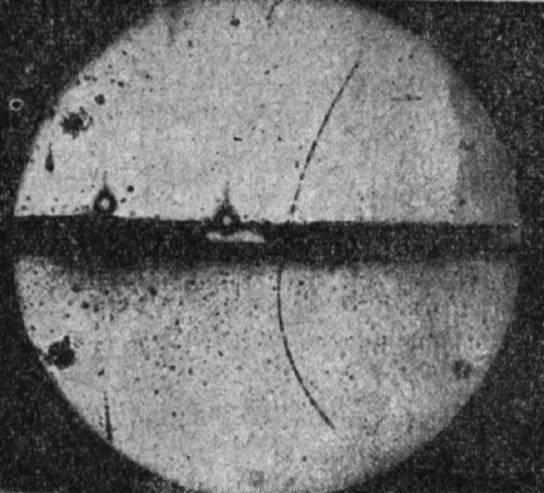
\includegraphics[width=7.0cm]{det01}
\end{floatingfigure}
Камера Вильсона сыграла выдающую роль в ядерной физике и физике
космических лучей. Ч.~Вильсон получил в~1927~г. Нобелевскую премию.
С~её помощью был, например, в~1932 году Андерсоном обнаружен позитрон
в космических лучах.
На протяжении нескольких десятилетий она была практически единственным
\footnote{В 40-е годы начались использоваться тоже ядерные эмульсии,
  которые применяются в экспериментах до сегодняшнего дня.} трековым
детектором. В~начале второй половины двадцатого века ей на замену
пришла пузырьковая камера.

\subsection{Пузырьковая камера}
Пузырьковая камера была изобретена Глэзером в 1952 году. Камера наполнена
перегретой жидкостью. Такая жидкость (обычно это жидкий водород)
неустойчива, и поэтому пролетающая через неё ионизирующая частица,
заставляет её мгновенно вскипать, вдоль пути частицы появляется цепочка
пузырьков пара. Перегретое состояние жидкости достигается резким
уменьшением давления. Камера становится на несколько миллисекунд
чувствительной (желательно это время синхронизовать со~временем
вхождения в камеру частиц из ускорителя). Образовавшийся, из цепочки
пузырьков пара, трек освещается и фотографируется. Заполняющая объём
жидкость, является одновременно и детектором и мишенью, это даёт
хорошую возможность получить почти полную картину взаимодействия.

Д. Глэзер в 1960 году получил за её изобретение Нобелевскую премию.
Развитие камер шло быстрыми темпами. В 70-х годов прошлого века они были
основными детекторами в физике высоких энергии. Рост энергий пучков
потребовал разработки камер огромных размеров.
Рабо- \newpage \noindent чий объём пузырьковых камер возрос почти
в миллионы раз \cite{har}.
\begin{figure}[h]\center
  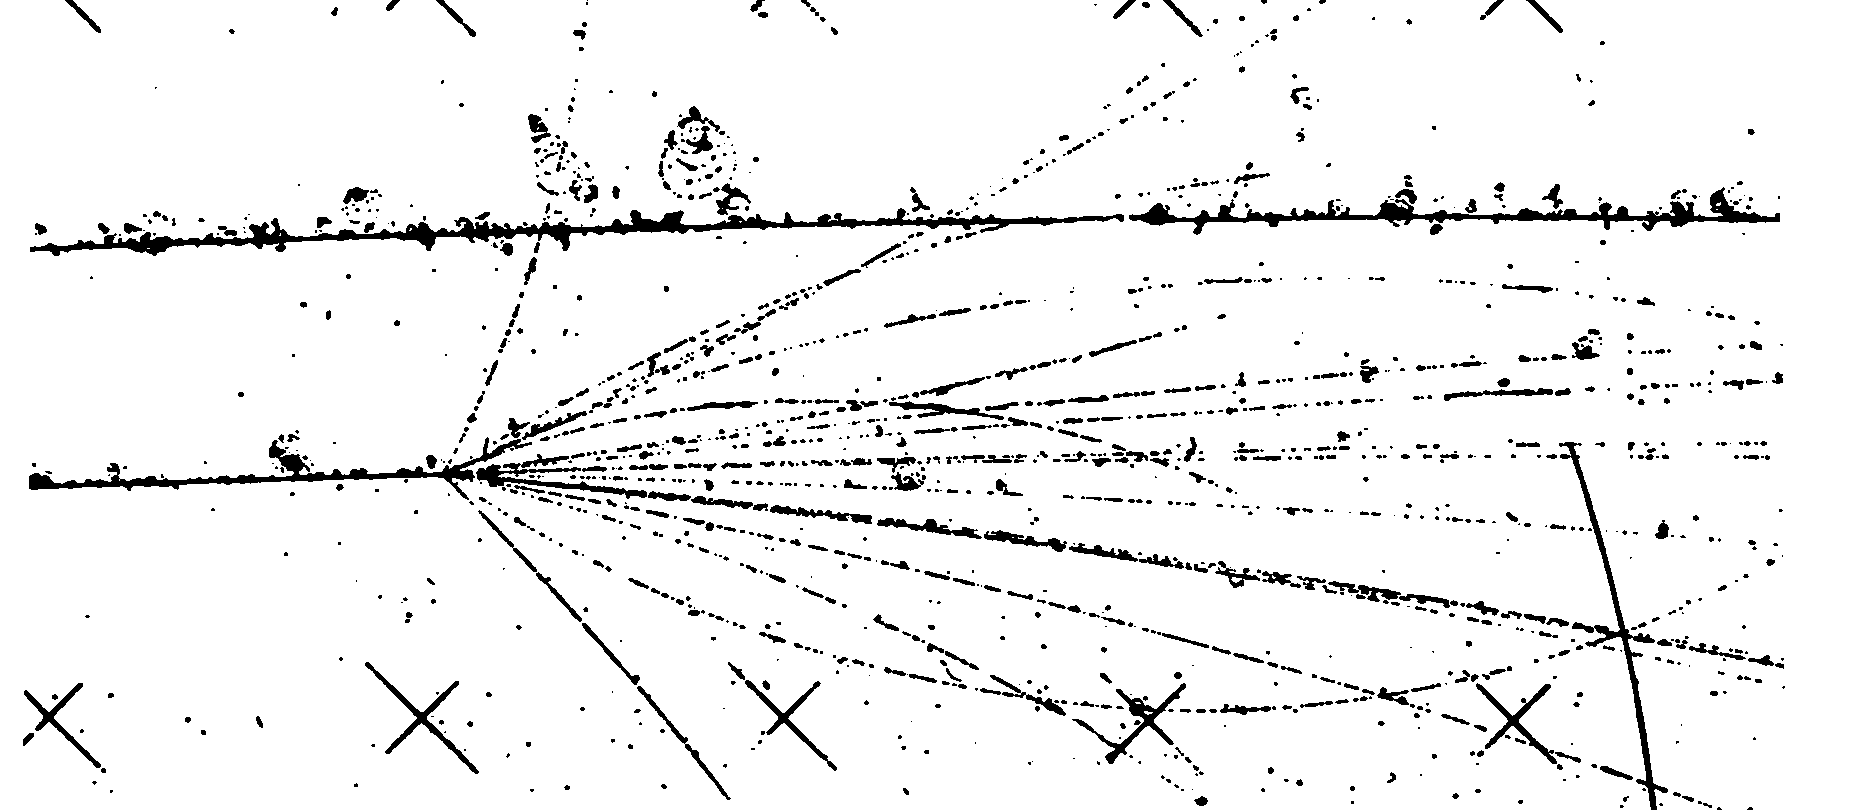
\includegraphics[scale=0.82]{det02}
  \caption{Полная дезинтеграция ядра фтора в водородной камере. Снимок из
    последнего сеанса 100-см водородной пузырьковой камеры ЛВЭ ОИЯИ
    в ноябре 1992 года \cite{gla}.}
\end{figure}

Несмотря на трудоёмкую работу связанную с расшифровкой фотографий
(восстановлением треков), основной недостаток пузырьковой
каме\-ры --- невозможность в процессе облучения выбрать интересующие нас
события, что приводит к необходимости просмотра большого количества
снимков.

\subsection{Искровая камера}
\begin{floatingfigure}[r]{0.20\textwidth}
  \vspace{-0.5cm}
  \hspace{-0.6cm}
  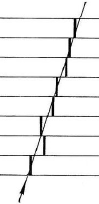
\includegraphics[width=0.18\textwidth]{det03}
\end{floatingfigure}
В конце 50-х годов прошлого века, появилась искровая камера. Она обычно
состоит из нескольких параллельных, плоских металлических пластин, которые
используются в качестве электродов. Пространство между ними заполняется
газом, чаше всего используется неон, гелий или аргон. Заряженная частица,
проходящая через камеру, образует ионы в газе. Одновременно (или
с маленьким опозданием $\sim$1 мкс), по сигналу совпадения из логического
устройства, обычно пара сцинтилляционных счётчиков, на электроды подаётся
короткий ($\sim$10-100 нс), высоковольтный ($\sim$10-20кВ/см) импульс
напряжения \cite{duk:04}. В~результате в месте прохождения частицы за
несколько наносекунд происходит видимый глазом искровой разряд\footnote{
  В стримерной камере, аналоге искровой камеры, формируются короткие
  светящиеся области, так называемые стримеры.}.
Возникающие искровые каналы фотографируются.

Искровая камера была хорошим дополнением к пузырьковой камере.
Появилась возможность управляемого запуска с помощью триггерных
счётчиков, для регистрации только нужных событий. Кроме того искровая
камера была способна работать более чем в сто раз чаще чем пузырьковая,
а~если время пролёта между частицами больше чем мёртвое время (время до
полного удаления заряда, образовавшего искры, оно приблизительно
несколько миллисекунд), то эффективность приближается к~100$\%$.

% Развитие, в это время вычислительной техники, позволило осуществить
% первые попытки замени оптической, фильмовой методики на электронный
% сбор данных.

\vspace{0.6cm}
\subsection{Ядерные фотоэмульсии}
Трек заряженной частицы можно регистрировать и методом аналогичным
обычному фотографированию. За развитие такого метода и открытия,
связанные с мезонами, сделанные с помощью фотографического метода
Ф.~Пауэлл в~1950~г. получил Нобелевскую премию.
\begin{floatingfigure}[r]{5.0cm}
  \hspace{-0.6cm}
  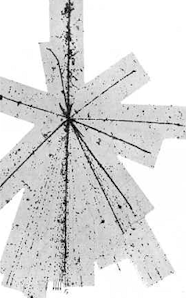
\includegraphics[width=4.8cm]{det04}
\end{floatingfigure}
Пластинки ядерных эмульсий состоят из мелких (0.2 $\div$ 0.3 мкм)
кристаллов бромида серебра, помещённых в слоях желатины \cite{nak:06}.
Отдельные слои складываются в стопку нужного объёма, обычно порядка
десятков сантиметров. Заряженная частица, проходящая через слои эмульсии,
вызывает химическое изменение в зёрнах бромида серебра, расположенных
вдоль трека ионизирующей частицы. Образуются зёрна металлического
серебра. Оставленный след в~фотоэмульсии просматривается микроскопом.
Отсюда и следует главный недостаток метода, очень трудоёмкая обработка
каждого слоя.

Однако, этот один из старейший методов регистрации частиц используется
до сих пор. В последнее время вновь возродилась техника фотоэмульсии.
Проводятся гибридные эксперименты, эмульсии вместе с электронными
детекторами, которые дают трековую информацию о нужном событии. Эта
информация потом упрощает, сокращает анализ эмульсии под микроскопом.

Высокое пространственное разрешение, порядка нескольких микрометров и
небольшая цена, являются основными преимуществами ядерных фотоэмульсии.

\subsection{Бесфильмовые камеры}
В начале второй половины XX века, во время быстрого развития ускорительных
комплексов, в физических экспериментах регистрации и локализации излучения
в ядерной и субъядерной физике встали две основные проблемы:
\begin{itemize}
\item неуправляемость детектора в процессе его работы, невозможность
  выделения интересующего нас события.
\item необходимость регистрировать информацию фотографическим
  способом. Извлечение данных из изображений треков, траекторий частиц,
  при огромном количестве фотоснимков оказывалось слишком трудоёмким.
  % (более миллиона в год, иногда и на один эксперимент)
\end{itemize}
Решение этих задач было сильно связано с начавшимся бурным развитием
транзисторной электроники, вычислительной техники. Появились методы
регистрации частиц с использованием ЭВМ, где информация сразу же
подвергалась математической обработке.

Разные комбинации счётчиков и методов регистрации, схемы совпадений
(антисовпадений) между событиями и т.п., позволили выделять разные,
интересующие нас события, частицы.

Первые попытки замены оптической, фильмовой методики на электронный
сбор данных появились уже у искровой камеры. Пластины были замени
проволочками, которые образовывали координатную сетку. Однако
невозможность управлять этой камерой чаще, чем приблизительно сто раз
в одну секунду, серьёзно сдерживали её применение.

Устранение этих недостатков, в том числе и решение проблемы
быстродействующего управляемого детектора, пришло с появлением
проволочных пропорциональных и дрейфовых камер. Бесфильмовые,
управляемые методы трековой регистрации частиц стали интенсивно
развиваться и широко использоваться. Кроме небольшого мёртвого времени,
которое экономит время работы ускорителя, проволочные пропорциональные
и дрейфовые камеры (и их модификации) обладают достаточно высоким
временным и пространственным разрешением.

Бесфильмовые камеры вместе с другими детекторами, цифровая (удобная)
информация, использование ЭВМ, быстрый анализ, всё это позволило
существенно увеличить скорость сбора экспериментальных данных в ядерной и
субъядерной физике на несколько порядков.

Рассмотрим ближе принцип работы основных представителей этой группы:
многопроволочных пропорциональных камер и дрейфовых камер.

\subsection{Ионизация в газовом детекторе}
\subsubsection{Подвижность и дрейф ионов}
Заряженная частица проходящая через рабочий объём детектора в результате
ионизации образует электроны и положительные ионы. Они быстро теряют
свою энергию при многократных столкновениях с атомами и молекулами газа,
распределение по энергии близко тепловому.

Со временем плотность образованного заряда уменьшается из за
рекомбинации --- нейтрализации положительных и отрицательных ионов и
электронного захвата --- возможности захватывать электроны низких энергий
некоторыми многоатомными молекулами. Вероятность такого захвата
характеризуется коэффициентом прилипания, который для
электроотрицательных газов, таких как $O_2, CO_2$ и $Cl_2$, достаточно велик,
но пренебрежимо мал для инертных газов $N_2, H_2, Ar$ и
$CH_4$ \cite{kla:90}.

Если образовавшиеся ионы подвергаются воздействию электрического поля
с напряжённостью $Е$, они начинаются двигаться вдоль линий электрического
поля.
\begin{floatingfigure}[l]{7.0cm}
  \hspace{-0.7cm}
  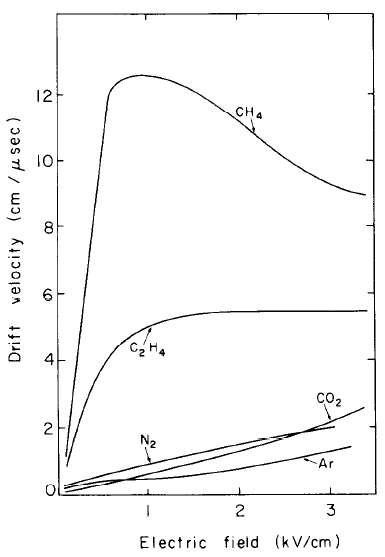
\includegraphics[width=6.7cm]{det05}
\end{floatingfigure}
\noindent
Средняя скорость движения электронов и ионов называется скоростью дрейфа,
её можно записать в виде: $v_d =\mu E$, где $\mu$ - подвижность ионов,
которая кроме напряжённости $Е$ в электрическом поле, зависит и от состава
газовой смеси, давления и температуры. На рисунке показана зависимость
скорости дрейфа электронов от напряжённости для некоторых смесей газа при
нормальных условиях.

Подвижность электронов в~газах приблизительно на три порядка больше чем
подвижность ионов.
% Ускорением ионов, электрическим полем, можно практически пренебречь.
Электроны, при достаточно большом значении напряжённости, смогут за
время между двумя столкновениями, приобрести в электрическом поле
энергию, достаточную для вторичной ионизации атомов газа, может произойти
газовое усиление. В результате число носителей зарядов возрастает.

%\subsubsection{Лавина электронов}
\subsubsection{Газовое усиление}
\begin{figure}[]\center
  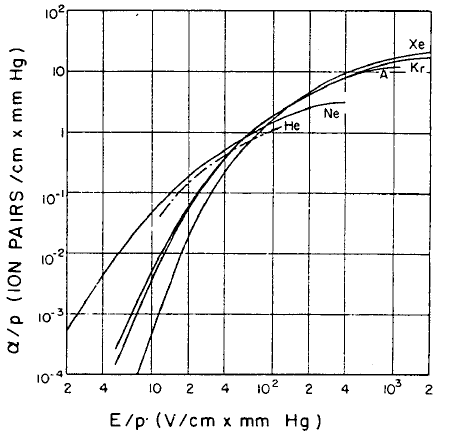
\includegraphics[scale=0.56]{det06}
  \caption{Первый коэффициент Таунсенда для разных инертных газов.}
  \label{fig:det06}
\end{figure}

При высоких значениях $E/p$, где $p$ - давление в газе, количество
вторичных электронов растёт лавинообразно. На рис.~\ref{fig:det06} видно,
что эффективное развитие лавины начинается в поле при $E/p \approx 100$
В/(см.мм рт.ст.) \cite{rop:04}.

Количество вторичных электронов в лавине $\alpha$\footnote{Зависимость
  $\alpha/p$ от $E/p$ (рис.~\ref{fig:det06}) можно описать эмпирическим
  выражением $\alpha/p = A~e^{-B(p/E)^k}$, где $A, B, k$ - константы газовых
  смесей.}, образованных одним электроном
на пути длины 1 см вдоль линии электрического поля,
называется первым коэффициентом Таунсенда, или коэффициентом ударной
ионизации. Если $N_0$ - число первичных электронов, созданных
ионизирующей
частицей, то полное число электронов $N(x)$ %собранных на аноде
в точке лавины~$x$ равно $N(x) = N_0~e^{\alpha x}$. Коэффициент газового
усиления можно определить как \cite{sau:02}:
\[
u~=~\frac{N}{N_0}~=~e^ {\int \alpha(x) \,dx}.
%u~=~\frac{N}{N_0}~=~e^{\int\limits_0^{x{_0}} \alpha(x)\,dx}.
\]
Если использовать инертные (благородные) газы, можно получить эффект
газового усиления и при более низкой напряжённости электрического поля.
В таких газах электрон в основном теряет энергию на их ионизацию, а не на
возбуждение.

%\subsubsection{Однопроволочный пропорциональный счётчик}
\subsubsection{Режимы работы газовых детекторов}
Зависимость собравшихся ионов на электродах детектора --- регистрируемый
заряд от величины напряжённости электрического поля для газонаполненного
цилиндрического детектора показана на рис.~\ref{fig:det07} \cite{leo:94}.
\begin{figure}[h]\center
  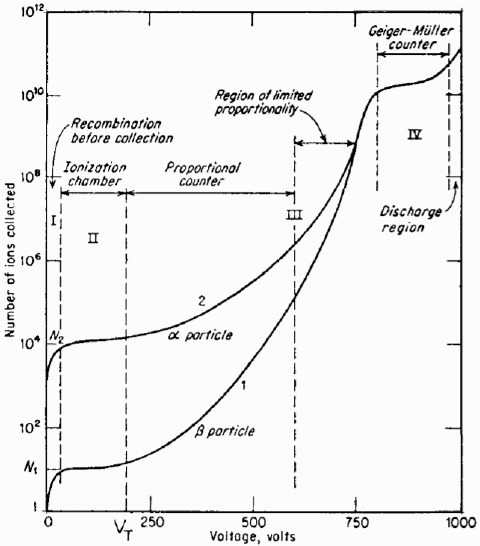
\includegraphics[width=10.8cm,height=11.2cm]{det07}
  \caption{Режимы работы газовых цилиндрических детекторов.}
  \label{fig:det07}
\end{figure}

В области напряжения I ионизации и собиранию заряда на электродах
препятствует процесс рекомбинации ионов. При увеличении напряжения
скорость ионов возрастает, рекомбинация уменьшается, амплитуда
возрастает.

В области II все образовавшейся ионы собираются на электродах. В этой
области работают ионизационные камеры.

При дальнейшем усилению напряжённости первоначальное число носителей
зарядов сильно возрастает, происходит газовое усиление. Участок III ---
область пропорционального режима. При более высоких электрических полях
образующийся заряд не будет зависит от первичной ионизации --- область
ограниченной пропорциональности.

В режиме работы счётчиков Гейгера-Мюллера, область IV,
% происходят огромные лавинообразный процесс,
регистрируемый сигнал становится одинаковым для частиц с различной
ионизацией (зависит только од напряжения). Регистрируется любая частица
способная создать хотя бы одну пару ионов в объёме счётчика.
%\subsubsection{Пропорциональный счётчик}

\subsection{Многопроволочные пропорциональные камеры}
Многопроволочная пропорциональная камера по сути представляет
набор цилиндрических пропорциональных счётчиков помешенных в одном
газовом объёме.
\begin{figure}[h]\center
  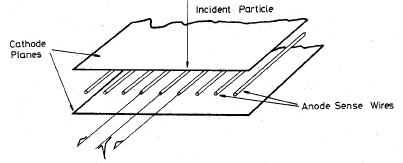
\includegraphics[scale=0.70]{det08}
  \caption{Схема конструкции многопроволочных пропорциональных камер.}
  \label{fig:det08}
\end{figure}
Схема такой камеры показана на рис.~\ref{fig:det08}. Между двумя
плоскими катодами из металлической фольги расположенные сигнальные
проволочки --- аноды (обычно это проволочки диаметром 20 мкм,
расположенные с шагом 2 мм).
\begin{figure}[h]\center
  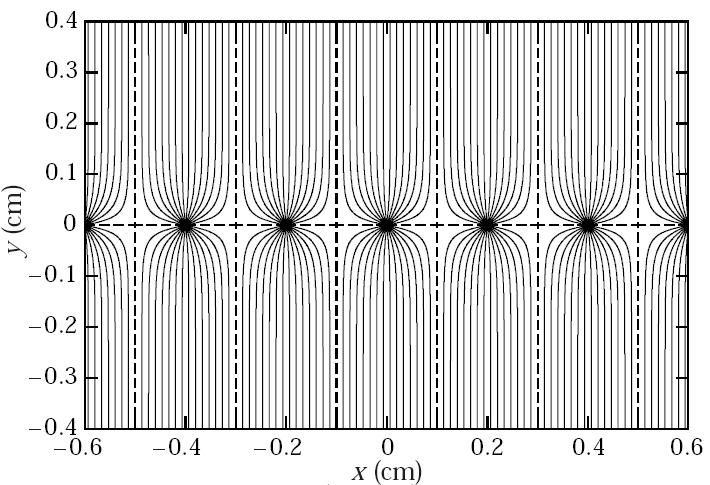
\includegraphics[width=10.8cm,height=6.2cm]{det09}
  \caption{Силовые линии электрического поля в пропорциональной камере
    с несколькими проволочками (симуляция программой GARFIELD \cite{gar}).}
  \label{fig:det09}
\end{figure}

Ионизирующая частица, проходящая через многопроволочную
пропорциональную камеру, образует вдоль своего пути свободные электроны,
которые зарождают лавины точно также, как и в пропорциональных счётчиках.
Заряд рождается в непосредственной близости от анодной проволочки
в области сильного электрического поля. Сигнал с каждой проволочки
регистрируется отдельно, что позволяет определить координату частицы
в камере.
\begin{figure}[h]\center
  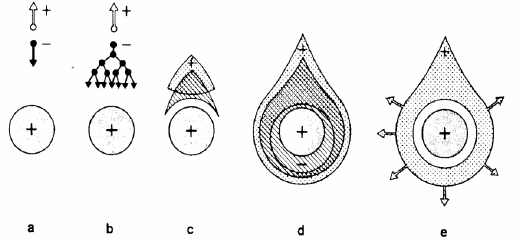
\includegraphics[width=12.0cm]{det10}
  \caption{Временно---пространственное развитие лавины вблизи анодной
    проволочки пропорциональной камеры.}
  \label{fig:det10}
\end{figure}

Поскольку большинство электронов рождается вблизи анода, они
проходят очень короткую область (несколько мкм) с малой разностью
потенциалов. Положительные ионы, дрейфующие в сторону катода, проходят
почти всю разность потенциалов. Это означает, что сигнал на анодной
проволочке создаётся, в основном, положительными ионами, а не
электронами \cite{pes:86}.

При конструкции многопроволочной пропорциональной камеры, желательно
чтобы диаметр анодной проволочки составлял приблизительно $1\%$ от
расстояния между ними, напряжённость электрического поля будет тогда
достаточной для газового усиления. В большинстве случаев в качестве анода
используются тонкие (диаметр от 10 до 30 мкм) вольфрамовые проволочки
гальванизированные золотом. Катодные плоскости обычно металлические
фольги или слои натянутых проволочек \cite{gru:99}.

При изготовлении камер, особенно больших размеров, электростатическое
отталкивание анодных проволочек приводит к проблеме их механической
нестабильности. Длинные проволочки нужно натягивать с большой силой, или
фиксировать на промежуточных расстояниях. Это в свою очередь приводит
к образованию локальных (неэффективных) зон в точке фиксации.

Пространственное разрешение камеры определяется в основном расстоянием
$d$ между проволочками. Среднеквадратичная ошибка вычисляется как
$\sigma = d/\sqrt 12$. Для типичного расстояния анодных проволок 2~мм,
погрешность определения координаты частицы, пересекающей камеру,
составляет $\sim 0.6$ мм. Уменьшение расстояния\footnote{Для получения
  нужного газового усиления, при уменьшении расстояния между
  проволочками, необходимо увеличивать напряжение.}
между анодными проволочками приводит к улучшению разрешения
% (кроме пространственного и временное).
Однако создание камер больших размеров с такими уменьшенными
межпроволочными расстояниями связано с рядом проблем, в том числе с
уже упомянутым электростатическим отталкиванием проволок.

Рабочие газы для пропорционального режима работы камеры должны иметь
высокий коэффициент газового усиления ---  инертные (благородные) газы.
В большинстве случаев используются аргон или ксенон с различными добавками,
в качестве которых чаще всего используются $CO_2, CH_4$, изобутан. С такими
смесями можно получить газовое усиление $\sim 10^5$ а эффективность
регистрации частицы близкая $100\%$. Использование так называемой
магической смеси ($75\%~Ar + 24.5\%~изобутана + 0.5\%~фреона$) позволяет
увеличить коэффициент газового усиления до $\sim 10^8$ \cite{zan:78}.

\subsection{Дрейфовые камеры}
Идея определения координаты частицы, вызывающей ионизацию газа,
измерением времени дрейфа первичных электронов в однородном
электрическом поле, была высказана уже вскоре после\footnote{
  Пропорциональные многопроволочные и дрейфовые камеры появились
  в 1968 году. Ж. Шарпак за вклад в открытие и создание детекторов
  получил в 1992 году Нобелевскую премию.}
появления многопроволочной пропорциональной камеры \cite{char:93}.

Разница во времени $\delta t$ определяется между моментом первичной
ионизации (прохождением частицы) $t_0$ и моментом, когда электроны
достигают анодной проволочки (попаданием облака заряда) $t_1$. Координату
$x$ места прохождения частицы можно вычислить с помощью следующего
выражения:
\[
x=\int_{t_0}^{t_1} v_d(t)\,\delta t
\]

Желательную постоянную скорость дрейфа $v_{d}$ можно достичь
образованием постоянной напряжённости электрического поля вдоль пути
дрейфующего электрона.
%Длина этой пути может достигать и несколько десятков сантиметров.
Между соседними анодными проволочками (находящимися под потенциалом
+ HV 2) вводятся дополнительные, потенциальные проволочки под
потенциалом - HV 1. На катодные проволочки подан распределённый
потенциал от 0 до - HV 1, рис.~\ref{fig:det11} \cite{sau:77}.
\begin{figure}[h]\center
  \hspace*{-0.2cm}
  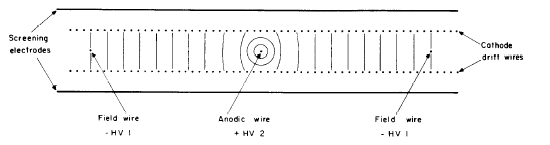
\includegraphics[scale=0.75]{det11}
  \caption{Схематический вид ячейки дрейфовой камеры с проволочными
    катодами.}
  \label{fig:det11}
\end{figure}

Пространственное разрешение дрейфовых камер определяется однородностью
электрического поля в области дрейфа. Как видно из рис.~\ref{fig:det12}
ограничение в разрешение вносит ещё временное разрешение электроники,
\begin{figure}[h]\center
  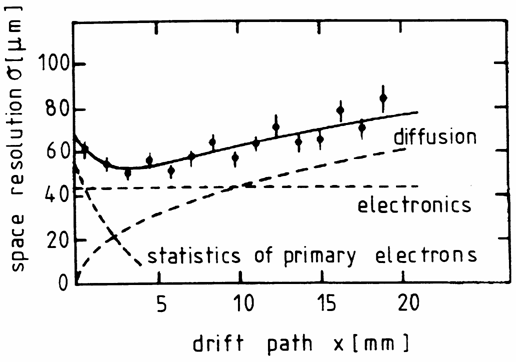
\includegraphics[scale=1.00]{det12}
  \caption{Зависимость пространственного разрешения дрейфовой камеры
    от пути дрейфа.}
  \label{fig:det12}
\end{figure}
диффузия электронов во время их дрейфа к аноду и статистическая
флуктуация первичной ионизации в близости анодной проволочки. Заметим,
что для частиц, проходящих под наклоном к плоскости камеры, разрешение
ухудшается (для очень больших наклонов почти в два раза).

\clearpage
\thispagestyle{plain}
\section{Заключение}
В представленном обзоре отражены лишь основные характеристики работы
газонаполненных координатно-трековых детекторов. Он не претендует на
полноту и не преследует цель охватить все развитые модификации
рассматриваемых устройств.

Упор сделан на пояснение принципов работы и происходящие физические
процессы при формировании сигналов от проходящих заряженных частиц.
В связи с этим в первой части обзора уделено внимание взаимодействию
частиц с веществом. Дана короткая информация о различных трековых приборах,
с их преимущества и недостатки с целью подчеркнуть ту нишу в детектировании
частиц, которая принадлежит газовым трековым детекторам.

\clearpage
\thispagestyle{empty}
\begin{landscape}
  \vspace*{1.3cm}
  \hspace*{-1.0cm}
  \large
  \begin{tabular}[c]{|p{6.0cm}|p{2.0cm}|p{1.8cm}|p{5.0cm}|p{5.0cm}|}
    \hline
    Трековый детектор & разреше\-ние [мкм] & мёртвое время [мс] &
    преимущества & недостатки
    \tabularnewline
    \hline
    \hline
    \slshape Камера Вильсона & 300 & $10^5$ & простота, первый трековый
    детектор & большое мёртвое время
    \tabularnewline
    \hline
    \slshape Пузырьковая камера & 20 & $10^2$ & анализ сложных
    событий & неуправляемость
    \tabularnewline
    \hline
    \slshape Искровая камера & 200 & $10$ & простота конструкции
    & низкая многотрековая эффективность
    \tabularnewline
    \hline
    \slshape Ядерная фотоэмульсия & 5 & 0 & пространственное
    разрешение, цена & трудоёмкий анализ событий
    \tabularnewline
    \hline
    \slshape Пропорциональные камеры & 200 & $10^-5$ & временное
    разрешение, простота & механическая нестабильность проволочек
    \tabularnewline
    \hline
    \slshape Дрейфовая камера & 50 & $10^-4$ & координатное
    разрешение & зависимость разрешения от диффузии и первичной
    ионизации
    \tabularnewline
    \hline
  \end{tabular}
\end{landscape}



%%% Local Variables:
%%% TeX-master: "referat"
%%% End:
